\documentclass[sigconf, nonacm]{acmart}
%% The following content must be adapted for the final version
% paper-specific
\newcommand\vldbdoi{XX.XX/XXX.XX}
\newcommand\vldbpages{XXX-XXX}
% issue-specific
\newcommand\vldbvolume{14}
\newcommand\vldbissue{1}
\newcommand\vldbyear{2020}
% should be fine as it is
\newcommand\vldbauthors{\authors}
\newcommand\vldbtitle{\shorttitle} 
% leave empty if no availability url should be set
\newcommand\vldbavailabilityurl{}
% whether page numbers should be shown or not, use 'plain' for review versions, 'empty' for camera ready
\newcommand\vldbpagestyle{plain} 


\newcommand{\red}{\textcolor{red}}
\newcommand{\techreport}{our technical report~\cite{techreport}}
\newcommand{\titlename}{Scalability and Efficiency of Graph Neural Networks}
% eat only in tech reports
\newcommand{\techreporteat}{}


%<*tag>

\usepackage{hyperref,array,color,balance,multirow}
\usepackage{balance,float,url,amsfonts,alltt}
\usepackage{mathtools,rotating,amsmath}

\usepackage{etoolbox,listings}
\lstset{basicstyle=\ttfamily\tiny,breaklines=true}
\usepackage{bigstrut,morefloats,pbox}
%\usepackage{amsmath}
\usepackage{graphicx,subfigure,xspace,verbatim,comment}
\usepackage{grffile}
\usepackage{ifpdf,fancyvrb}
\usepackage{algorithm}
\usepackage[noend]{algorithmic}
\usepackage{booktabs}
\usepackage{lipsum}  
\usepackage[all]{nowidow}
\usepackage{multirow}
\usepackage{pifont}
\usepackage{xcolor}

\newtheorem{theorem}{Theorem}[section]
\newtheorem{proposition}{Proposition}[section]
\newtheorem{corollary}[theorem]{Corollary}
\newtheorem{lemma}[theorem]{Lemma}
\newtheorem{definition}{Definition}[section]
\newcommand{\eat}[1]{}
\newcommand{\system}{Cerebro on Data Systems}
 \newcommand{\eqdef}{=\mathrel{\mathop:}}
 \definecolor{mygreen}{HTML}{3EC300}
\newcommand{\cmark}{{\color{mygreen} \ding{51}}}%
\newcommand{\xmark}{\color{red} \ding{55}}%

\DeclareMathOperator*{\gammasum}{\scalerel*{\Gamma}{\sum}}
\usepackage{scalerel}

%\DeclarePairedDelimiter{\ceil}{\lceil}{\rceil}

\newenvironment{packeditems}{
\begin{itemize}
  \setlength{\itemsep}{1pt}
  \setlength{\parskip}{0pt}
  \setlength{\parsep}{0pt}
}{\end{itemize}}

\newenvironment{packedenums}{
\begin{enumerate}
  \setlength{\itemsep}{1pt}
  \setlength{\parskip}{0pt}
  \setlength{\parsep}{0pt}
}{\end{enumerate}}

%\newcolumntype{P}[1]{>{\centering\arraybackslash}p{#1}}

\newtoggle{TR}
%\toggletrue{TR}

\DeclareMathOperator*{\argmin}{arg\,min}


\begin{document}\sloppy
\title{\titlename}



%\numberofauthors{8}
\author{Yuhao Zhang}
\affiliation{%
\institution{University of California, San Diego}
}
\email{yuz870@eng.ucsd.edu}



\begin{abstract}
A brief survey of GNN systems.

\end{abstract}
\maketitle

\pagestyle{\vldbpagestyle}
\techreporteat{
%%% do not modify the following VLDB block %%
%%% VLDB block start %%%
\begingroup\small\noindent\raggedright\textbf{PVLDB Reference Format:}\\
Yuhao Zhang. \vldbtitle. PVLDB, \vldbvolume(\vldbissue): \vldbpages, \vldbyear.\\
\href{https://doi.org/\vldbdoi}{doi:\vldbdoi}
\endgroup
\begingroup
\renewcommand\thefootnote{}\footnote{\noindent
$^*$Work was done when the author was at VMware, Inc.\\
This work is licensed under the Creative Commons BY-NC-ND 4.0 International License. Visit \url{https://creativecommons.org/licenses/by-nc-nd/4.0/} to view a copy of this license. For any use beyond those covered by this license, obtain permission by emailing \href{mailto:info@vldb.org}{info@vldb.org}. Copyright is held by the owner/author(s). Publication rights licensed to the VLDB Endowment. \\
\raggedright Proceedings of the VLDB Endowment, Vol. \vldbvolume, No. \vldbissue\ %
ISSN 2150-8097. \\
\href{https://doi.org/\vldbdoi}{doi:\vldbdoi} \\
}\addtocounter{footnote}{-1}\endgroup
%%% VLDB block end %%%

%%% do not modify the following VLDB block %%
%%% VLDB block start %%%
\ifdefempty{\vldbavailabilityurl}{}{
\vspace{.3cm}
\begingroup\small\noindent\raggedright\textbf{PVLDB Artifact Availability:}\\
The source code, data, and/or other artifacts have been made available at \url{\vldbavailabilityurl}.
\endgroup
}
}
%%% VLDB block end %%%




\section{Overview}
\subsection{Compared systems}
GNN systems are designed to execute (and scale) GNN workloads.  Some of them focus on single-node execution and optimizing data movement across memory hierarchy; some focus on distributed settings and optimizing network communications and graph partitioning. The usual goals are better runtime efficiency, measured as per-epoch training time, and data/model scalability, tested by the system being capable to execute the workload without OOM issues. This is an emerging field and many of these systems are still under active development and changed rapidly.

Although there are many sub-branches in GNN study, the vast majority of these systems focus on the spatial-based methods, that is, recurrent GNNs and spatial-based graph convolutional neural networks (also known as GCNs). Majority of spatial methods can be expressed via a general update rule:
\begin{gather}
\label{eq:mp}
\mathbf{h}_v ^k = \psi ( \mathbf{x}_v^k, \gammasum_{u \in {\mathcal {N}}(v)}  \phi(\mathbf{h}_v^{k-1}, \mathbf{h}_u^{k-1}, \mathbf{x}_{e_{vu}})),
\end{gather} 
where $\psi$, $\phi$, $\Gamma$ are potentially learnable and differentiable functions, $\Gamma$ is typically further required to be commutative and associative. $\psi$ is called the update function, $\phi$ the message function and $\Gamma$ the aggregate function. $\mathbf{h}_v^{k}$ is the node embedding for node $v$ at the $k$-th layer. $\mathcal {N}(v)$ is a function that returns all the neighbors for node $v$. $\mathbf{x}_{e_{vu}}$ is the edge feature.

\begin{figure*}[t]
 \centering
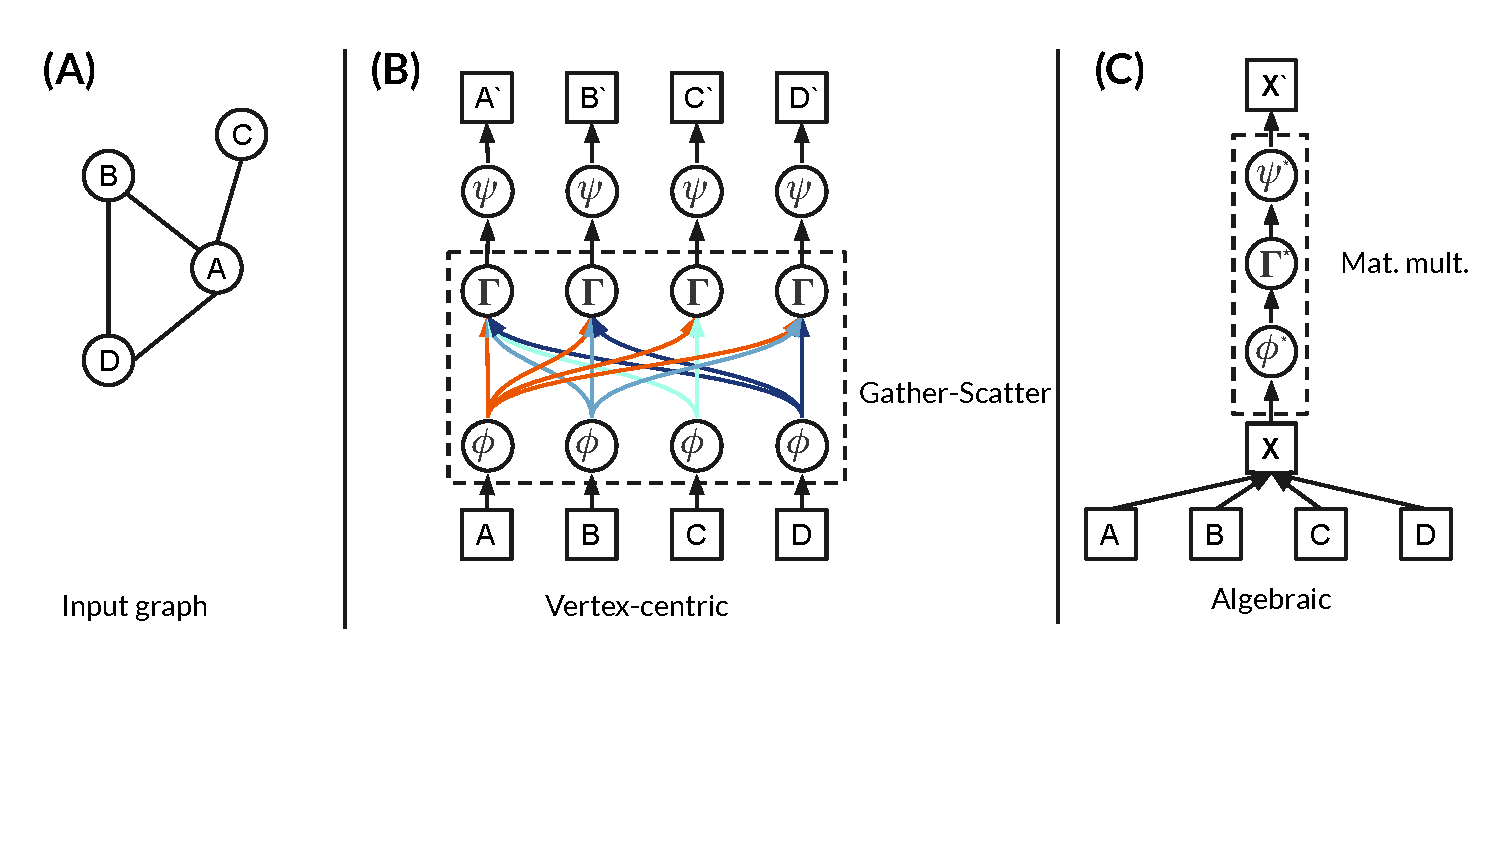
\includegraphics[width=0.70\textwidth]{./images/gnnsys.pdf}
 \caption{An example of two different approaches for GNN execution. (A): Input graph. (B): Vertex-centric approach. (C): Algebraic approach.}
 \label{fig:gnnsys}
\end{figure*}

\vspace{2mm}
\noindent \textbf{PyTorch Geometric (PyG)}  
Equation~\ref{eq:mp} fits in the paradigm of vertex-centric programming, which is a common programming model in the graph processing world~\cite{vertexcentric, powergraph, pregel} and very easy to parallelize. One of the first GNN systems, PyG~\cite{pyg} follows this pattern and builds GNNs as dataflow graphs on top of PyTorch~\cite{torch}, a dataflow system. Figure~\ref{fig:gnnsys} (B) shows an example computational graph generated\footnote{Note this observation is based on the published paper of PyG, in the recent versions of the release, PyG has implemented support for algebraic approach as well}. Each (vectorized) operation is then put on a separate processor to achieve parallelism. Built on top of PyTorch, PyG can easily utilize the features PyTorch provides, such as autograd, GPU acceleration, etc. 

\vspace{2mm}
\noindent \textbf{Deep Graph Library (DGL) and DistDGL.}  
Arguably the most popular GNN system, DGL~\cite{dgl} takes a different approach for the GNN execution, especially for the message passing (gather-scatter) part. It takes an algebraic approach for the execution by expressing GNN as sparse matrix multiplications (SpMM). This is analogous to those algebraic approaches to general graph analytics tasks~\cite{graphla}.

Figure~\ref{fig:gnnsys} (C) gives an example of the algebraic approach taken by DGL; each step is summarized as linear algebra and executed as SpMM, which is executed via DGL's own specialized kernel. DGL is built upon existing deep learning systems, and the user can also write user-defined functions to extend the built-in functions. DGL describes itself as a framework independent system, that is, independent of the underlying deep learning system. It has full support for several popular frameworks such as Tensorflow or PyTorch as backend. Backpropagation can also be done via another SpMM, and DGL functions are registered in the underlying deep learning framework to take advantage of autograd.

The algebraic approach opens possibilities of operator fusion. For many GNNs, the message function and aggregate function can be represented with purely matrix multiplications. Note in this form, the message function can be fused together with the aggregation function, and there is no need to materialize the intermediate messages, thus saving space. For scalability, DGL goes for distributed processing as DistDGL~\cite{distdgl}.

\vspace{2mm}
\noindent \textbf{NeuGraph.}
NeuGraph~\cite{neugraph} is another GNN system built on top of a dataflow system and designed for a single-node multi-GPU setting. It extends the GAS~\cite{powergraph} programming model and partitions the graph into chunks. It feeds chunks, instead of full graph to GPU, avoiding GPU OOM issues for GNNs without sampling the data. After feedforward propagation, chunks are swapped back to main RAM. There are also a series of processing order and scheduling challenges that it tries to solve. It further exploits GPU-to-GPU communication to avoid latencies of GPU-to-DRAM. 

\vspace{2mm}
\noindent \textbf{PaGraph.}
PaGraph~\cite{pagraph, pagraph2} also targets single-node multi-GPU setting and claims that the majority of the time (74\%) during GNN training is spent on data movement between the main RAM and GPU memory. Therefore to reduce such data movement, they utilize the spare GPU memory to statically cache certain graph nodes' features. They select this set of cache based on the nodes' degree. They then proposed a GNN-aware graph partition scheme for multi-GPU support. This partition scheme would ensure that each partition contains all of the training graph nodes' K-hop neighbors by replication. In a subsequent work~\cite{pagraph2}, the authors also incorporated pipelining. PaGraph is built on top of DGL and PyTorch.

\vspace{2mm}
\noindent \textbf{AliGraph.} 
AliGraph~\cite{aligraph} is one of the early distributed GNN systems that come with only CPU support. The paper proposes both a GNN training platform and a GNN algorithm to tackle real-world e-commerce graph analytics challenges. On the system side, they propose to store the graph structural information and node features data separately. AliGraph then use indices to represent the node features, therefore reduces the storage cost. They then adopt a LRU cache to reduce access time for the most frequent graph nodes that are also above a threshold based on their degrees. Furthermore, they adopt a lock-free distributed data structure (with cache) facilitate graph sampling that is common in GNN training.

\vspace{2mm}
\noindent \textbf{ROC.} 
ROC~\cite{roc} is a distributed GNN system that attempts to boost both the efficiency and scalability of GNN training. Towards the former goal, it adopts a ML-based method for determining the graph partition. For the later goal of scalability, it proposes system DRAM spill when the GPU memory is insufficient to execute the GNN workload. ROC is built upon an custom-built DNN execution backend with customized CUDA kernels, FlexFlow~\cite{flexflow}.


\vspace{2mm}
\noindent \textbf{P$^{3}$.} P$^{3}$~\cite{pcube} is a distributed GNN system that proposes to use a ``hybrid" parallelism for GNN training. They argue that under the distributed setting, training time is dominated by the communication time. They also claim that the bulk of communication happens during the first layer of GNNs. P$^{3}$ then proposes to 1. partition the graph structure and node features independently. 2. partition the node features uniformly along the dimensions. This way they execute GNNs' first layer via model parallelism since each machine contains only several dimension of the features. They then invoke all-to-all communications and let each machine pull all the needed features, then proceed as normal data parallelism for subsequent layers. This execution scheme would bring extra overhead compared to simple data parallelism, but the authors argue such overheads are compensated by the performance gain brought by communication reduction.



\vspace{2mm}
\noindent \textbf{DeepGalois.} 
DeepGalois~\cite{deepgalois} is a CPU-only distributed GNN system built on a graph processing system Galois~\cite{galois}. Additionally, it is also built on top a series of existing graph partitioning and distributed communication framework. Because of these mature components, DeepGalois can support many graph partitioning scheme and can outperform distDGL. At the moment, there is not a full paper about DeepGalois and no public release can be found.


\vspace{2mm}
\noindent \textbf{Neo4j, TigerGraph, and GraphScope.}
Both Neo4j~\cite{neo4j} and TigerGraph~\cite{tigergraph} are graph DBMSes that have some GNN training capabilities. GraphScope~\cite{graphscope} is a recent graph processing system that primarily focuses on traditional graph analytics such as community detection, paths and connectivity, and centrality, but it also has extensible connecters to other systems to enable GNN processing.

Neo4j has implemented a specialized in-memory graph store for GNNs and other more advanced analytics. At runtime, it first moves data from the graph DB to this store and invokes custom-built library for building GNN model and SGD training. As of now, it only supports GraphSage. 

GraphScope takes a similar approach to Neo4j by moving data to a dedicated GNN facility. But instead of a custom-built framework, it can utilize TensorFlow and provides a few pre-built implementations of several popular GNNs.

TigerGraph, similar to Neo4j, only provides limited GNN support for simple GCNs. However, it takes a different approach by also storing all the NN neurons in graph DB. As mentioned above, such GNNs can be captured under the GAS abstraction. This way the GNN can be expressed mostly in the form of graph DB operators, instead of external library's dataflow operators. Forward and backward propagation can be written using TigerGraph's DSL: GSQL. Gradient computing is implemented in the form of UDFs.


\subsection{Other related systems}

\vspace{2mm}
\noindent \textbf{Custom-built, Specialized GNN Frameworks.} Due to the lack of support for GNNs from the commonly used deep learning frameworks such as TensorFlow and PyTorch and various other reasons, many ML researchers sought to build their own library for their specific GNNs/applications~\cite{agl, graphsage}. These frameworks usually are very specific and have little consideration for system performances such as efficiency and scalability. Therefore, they are excluded from our discussion.


\vspace{2mm}
\noindent \textbf{Knowledge Graph Embedding Systems.} There exists a connected, yet still different field of knowledge base graph embedding systems~\cite{marius, dgl-ke, pbg, lightne}. The goal of such systems is to obtain embeddings for each node within the graph. However, instead of training a GNN and using its internal latent node representations as node embeddings, these methods train the embeddings directly using the graph's structural information. They do not use GNNs and they usually work on graphs that are not featured, i.e., node and edge features unavailable. These systems also face efficiency and scalability challenges, mostly brought by the sheer size of knowledge base graphs, instead of GNNs. Many of them sought to use distributed processing, intelligent caching, and disk-aware processing to tackle these problems. Some of the techniques can be adopted for GNN systems, but many are specific to knowledge graph embedding workloads.

%----------------------------------------------
\begin{table*}[h]
\caption{Overview of comparisons.}
\scalebox{0.58}{
\huge{
\begin{tabular}{@{}ccccccccccc@{}}
\toprule
\multirow{2}{*}{} & \multirow{2}{*}{License} & \multirow{2}{*}{GPU} & \multicolumn{4}{c}{Efficiency}                                          & \multicolumn{2}{c}{Scalability} & \multirow{2}{*}{Expressibility} & \multicolumn{1}{l}{\multirow{2}{*}{Memory Hierarchy}} \\ \cmidrule(lr){4-9}
                  &                          &                      & Data movement & Communication & Training & \multicolumn{1}{c|}{Overall} & Distributed      & Sampling     &                                 & \multicolumn{1}{l}{}                                  \\ \midrule
PyG~\cite{pyg}               & Open                     & Yes                  & -             & N/A           & +        & -       & No               & Generic      & GAS                             & GPU-only                                              \\
DGL~\cite{dgl, distdgl}               & Open                     & Yes                  & -             & -             & +        & -       & Yes              & Generic      & MM                              & GPU-only                                              \\
NeuGraph~\cite{neugraph}          & N/A                      & Yes                  & ++            & N/A           & +        & +       & No               & GD           & GAS                             & Main-aware                                            \\
PaGraph~\cite{pagraph, pagraph2}           & Open                     & Yes                  & ++            & N/A           & +        & ++      & No               & SGD          & MM                              & Main-aware                                            \\
AliGraph~\cite{aligraph}          & Open                     & No                   & +             & +             & -        & -       & Yes              & SGD          & GAS                             & Main-only                                             \\
ROC~\cite{roc}               & Open                     & Yes                  & +             & +             & +        & ++      & Yes              & GD           & GAS                             & Main-aware                                            \\
P$^{3}$~\cite{pcube}           & N/A                      & Yes                  & -             & ++            & -{}-       & ++      & Yes              & SGD          & MM*                             & GPU-only                                              \\
DeepGalois~\cite{deepgalois}        & N/A                      & No                   & -             & +             & -        & +       & Yes              & GD           & GAS                             & Main-only                                             \\
Neo4j~\cite{neo4j}             & Mixed                    & No                   & -{}-            & N/A           & -        & -{}-      & No               & SGD          & ?                               & Main-only?                                            \\
TigerGraph~\cite{tigergraph}        & Closed                   & No                   & -             & -             & -        & -       & Yes?             & GD?          & GAS?                            & Main-only?                                            \\
GraphScope~\cite{graphscope}        & Open                     & Yes                  & -{}-            & ?             & -        & -       & No?              & Generic?     & ?                               & GPU-only?                                             \\ \bottomrule
\end{tabular}
}
}
\label{tab:comp}
\end{table*}

\vspace{-2mm}
\section{Comparisons of GNN systems}
An overview of all the systems compared is shown in Table~\ref{tab:comp}.
\label{sec:comp}
\subsection{Availability (licenses)}
For the purpose of benchmarking and development on top of these systems, ideally we want them to be free and open-sourced.


\vspace{2mm}
\noindent \textbf{Open-source license.}
Majority of the GNN systems surveyed are open-sourced, exceptions are below.


\vspace{2mm}
\noindent \textbf{Proprietary license.}
TigerGraph is released under a proprietary license, the free version comes with a limitation of graph storage size. Neo4j, on the other hand, has both a free open-sourced version that comes with various limitations, and a paid commercial version.

\vspace{2mm}
\noindent \textbf{Not available.}
There are no public releases found for NeuGraph, DeepGalois and P$^3$.




\subsection{Accelerator (GPU) Support}
With GPU support, two extra problems arise: 1. efficient data movement between main memory and GPU memory 2. memory management to prevent crashes, as GPU RAM is usually more limited. Not all systems have GPU support.

\vspace{2mm}
\noindent \textbf{GPU-supported.} PyG, DGL, NeuGraph, PaGraph, ROC, P$^{3}$, and GraphScope all support GPU training. Among which, PyG, DGL, and ROC have custom-built GPU kernels for GNNs. The rest are based on existing systems for GPU support.

\vspace{2mm}
\noindent \textbf{CPU-only.} AliGraph, DeepGalois, Neo4j, and TigerGraph are CPU-only at the moment.

\subsection{Runtime Efficiency (Speculated)}
This section is based on the published results from the papers. These results are not directly comparable, as they are not done on the same platform, nor the same datasets/models. Hence, currently without more rigorous tests, the efficiency can only be speculated. There are many aspects to the runtime efficiency: 1. data movement efficiency across memory hierarchy, pipelining, and efficiency latency hiding. 2. for distributed systems, the network communication efficiency, graph partitioning quality, cache, and novel parallelization schemes. 3. actual training efficiency, i.e., runtime spent in GPU. 

In the literature, the more common baselines are DGL and PyG. Between the two, both of their papers claim to be faster and more scalable, it is unknown if they have a substantial gap in performance.

\vspace{2mm}
\noindent \textbf{Data movement efficiency.}
A few systems have efforts in optimizing the data movement, especially the DRAM-GPU movement. The common techniques are caching and pipelining. NeuGraph, ROC, and PaGraph all adopt some form of caching to reduce the data movement and try to overlap computation with data transfer. NeuGraph further exploits opportunities for GPU-GPU data movement.

\vspace{2mm}
\noindent \textbf{Network communication efficiency.} Networking becomes part of the problem when distributed processing comes to picture. AliGraph and ROC both consider graph partitioning algorithm, and caching, to boost data locality and reduce communication. DeepGalois relies on the underlying graph processing software stack for optimized graph partitioning and distributed communication. P$^{3}$, on the other hand, proposes a parallel execution scheme that mixes model parallelism and data parallelism, to reduce communications.

\vspace{2mm}
\noindent \textbf{Training efficiency.} Most of the systems should have close performance in this department. However, as PyG, DGL, NeuGraph, and ROC all have their custom-made GPU kernels for graph propogation, it is unknown which one is the winner as no such drill-down benchmark is currently available. In addition, P$^3$ adopts a model parallelism training scheme that is different from all other systems and this scheme, although may save communications, but would likely add overheads to training.



\subsection{Scalability (Speculated)}
Due the neighborhood explosion problem and the scale of large graphs, GNNs suffer from scalability issues as the entire graph is usually much larger than the GPU memory can hold. A series of algorithmic efforts, focusing on sampling, have been proposed to mitigate this issue. However, even with mini-batch SGD and sampling over the data, it is claimed that many of such workloads can still face scalability issues. Common techniques include 1. distributed processing that enables multi-GPUs, and 2. spilling to main RAM to prevent OOM. Distributed processing would lead to topics such as graph partitioning, network communication, and parallel schemes. Spilling to main RAM is tightly connected to topics such as caching and pipelining.

\vspace{2mm}
\noindent \textbf{Distributed processing.} DGL, ROC, DeepGalois, P$^{3}$, AliGraph, and TigerGraph can all support distributed GNN training. PyG, NeuGraph, PaGraph are single-node systems.

Neo4j and GraphScope are unknown if their export-based methods can be made distributed. Apart from this, Neo4j is currently still primarily a single-node and not fully distributed graph DB\footnote{https://neo4j.com/news/neo4j-going-distributed-with-graph-database/}.

\vspace{2mm}
\noindent \textbf{Graph sampling.} 
There are mainly two categories of systems in terms of graph sampling and training scheme: full-batch and mini-batch.
\begin{enumerate}
\item \textbf{Full-batch. (Gradient descent and unsampled)}.
The first try to optimize for full-batch training of GNNs, i.e. naively would require the entire graph to fit in the main or GPU RAM. This category includes NeuGraph, ROC, and DeepGalois. TigerGraph currently has some support for GCNs and can work under full-batch setting. However, it is unknown to what extend it is scalable.
\item \textbf{Mini-batch. (SGD and sampled)}. The second category assumes mini-batched and sampled graph, therefore they only require a mini-batch of data to fit in the RAM. This category includes PaGraph, AliGraph, and P$^{3}$. Neo4j only supports GraphSage algorithm at the moment, which is a mini-batch method with sampling. 
\item \textbf{Generic. (Unspecified)}. These systems claim to be generic or not specifically optimized for any one particular setting. It includes DGL, PyG, and GraphScope.
\end{enumerate}
Technically the first category should be able to also work under the mini-batched setting, but the reverse may not be true.  


\subsection{GNN Expressibility}
\begin{figure}[t]
 \centering
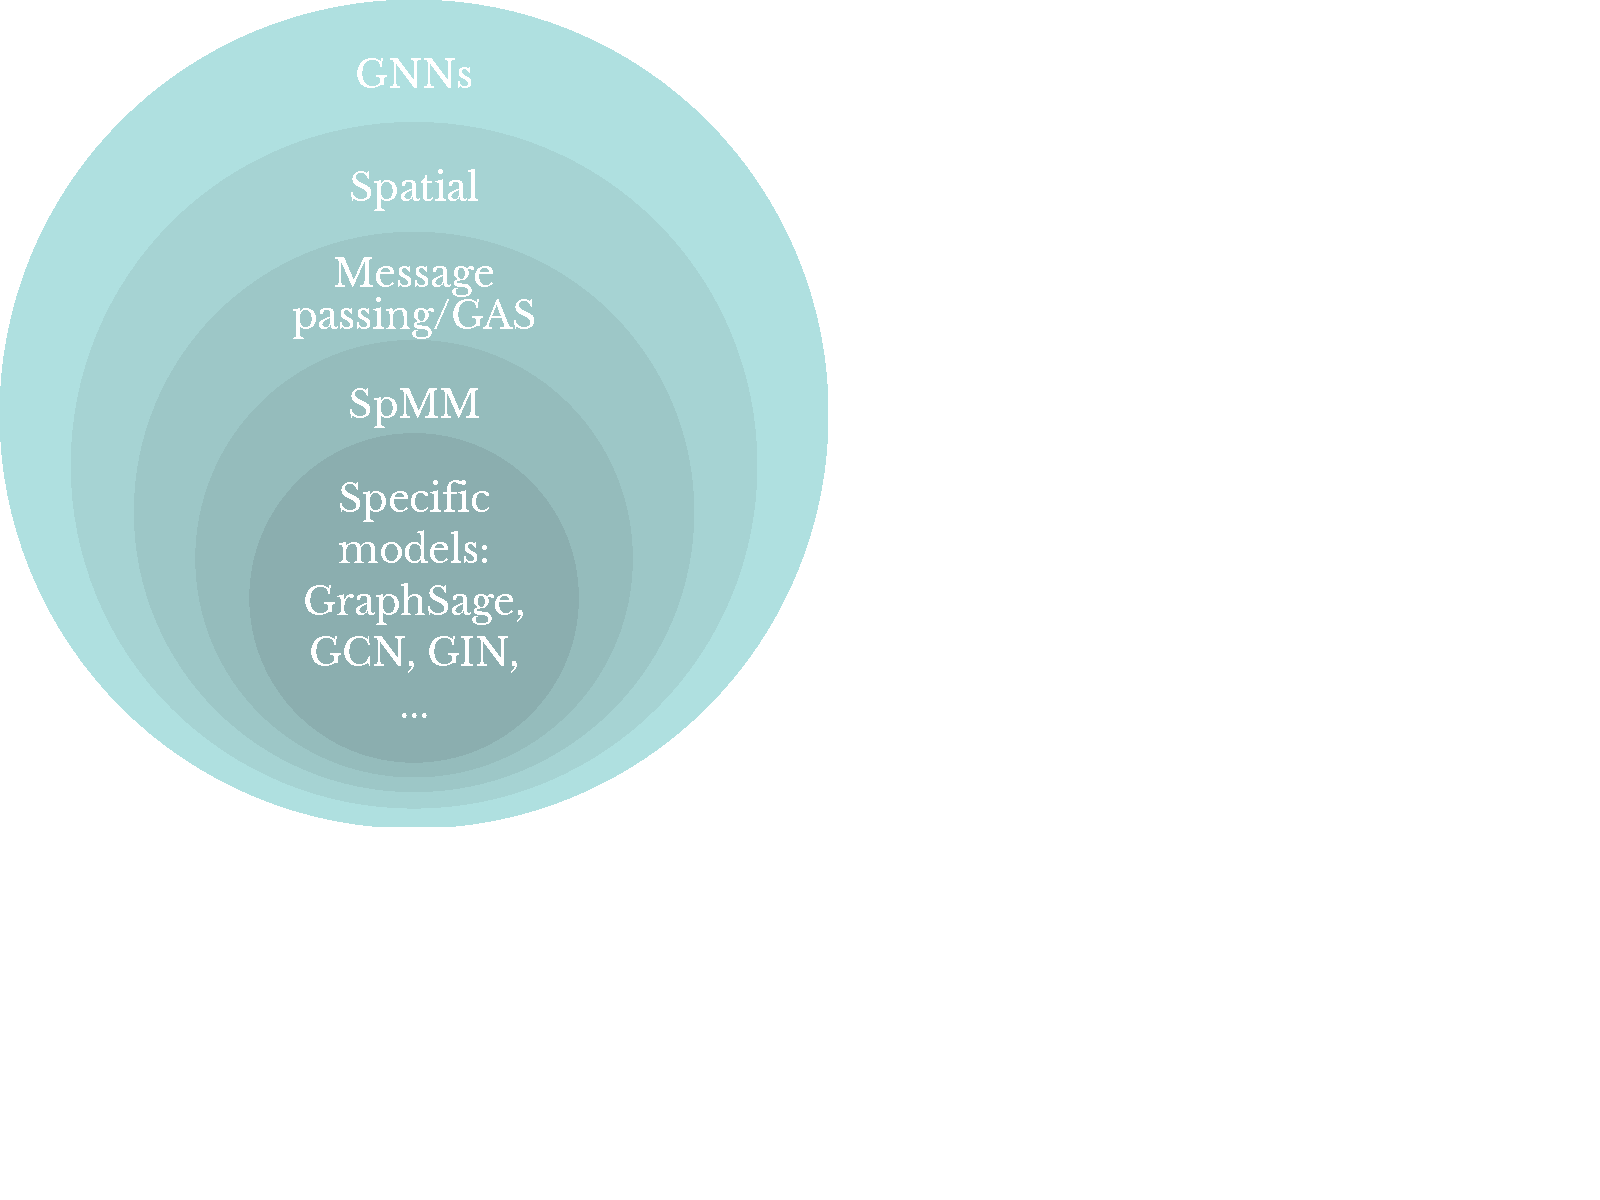
\includegraphics[width=0.35\textwidth]{./images/venn_diagram.pdf}
 \caption{Venn diagram of different scopes of GNNs.}
 \label{fig:venn}
\end{figure}


We now evaluate how generic are these systems and the family of GNN models that can be expressed/executed by these systems. Figure~\ref{fig:venn} shows the overall scope of comparisons. 
\begin{itemize}
\item First, all of these systems are primarily designed for spatial methods, most of the spectral-based GNNs are well-supported, except a few methods like ChebNet~\cite{chebnet} that bridges the spectral- and spatial-based GNNs. 
\item Furthermore, many systems are based on the message passing interface shown in Equation~\ref{eq:mp}, also can be captured under the GAS framework. Such systems include PyG, NeuGraph, AliGraph, ROC, and DeepGalois.
\item DGL further requires the GNN to be expressible as matrix multiplications. PaGraph is built on top of DGL, so it shares the same expressibility. On the other hand, for P$^{3}$ to show performance gain, the update function of the model needs to be model-parallelizable, that usually means linear operations/simply matrix multiplications.
\item Neo4j, TigerGraph, and GraphScope did not focus on the GNN expressibility and are unknown how general their programming interface is, or they do not have a generic programming interface for expressing various GNN models. 
\end{itemize}

\subsection{Span of Memory Hierarchy}
We now inspect each system's usage of different memory hierarchy, from accelerator memory all the way to disk. Generally speaking, the wider the span is, the better the system can scale with large model and data. Not all systems support GPUs, so some of them cannot span to GPU RAM. But as more tiers hierarchy are involved, the latencies grow and the demand for buffering and memory management also grow.

\vspace{2mm}
\noindent \textbf{GPU RAM Only.} DGL, PyG, and P$^{3}$ are GPU RAM only, meaning they require the full graph/minibatch to fit in the memory.


\vspace{2mm}
\noindent \textbf{Main RAM Only/Aware.} AliGraph and Neo4j are main RAM only. NeuGraph, PaGraph, and ROC all utilize the main memory and spill intermediate results to it. They have different strategies to handle the main-memory to GPU data movement. All of the above require the data, GNN model, and intermediate results to fit in the main memory.

\vspace{2mm}
\noindent \textbf{Disk Aware.} At the moment, there is no systems that explicitly claim that they are disk aware. Neo4j and TigerGraph, as graph DBs, have disk spilling capability for the DB part. However, neo4j processes GNN workloads in a strictly in-memory store, while it is unclear whether TigerGraph can spill GNN intermediate states to disk. GraphScope, on the other hand, replies on external libraries for GNN execution and can be flexible.







%\begin{table}[t]
\centering
\caption{Notations used in this paper.}
\scalebox{0.90}{
\begin{tabular}{@{}ll@{}}
\toprule
Notation & Description \\ \midrule
$G(V, E)$     & A graph $G$ with nodes set $V$ and edges set $E$        \\
$v, e$     & Node and edge        \\
$\mathbf{x}_v, \mathbf{x}_e$     & Node and edge features of $v$ and $e$, respectively      \\ 
$\mathbf{X}_V, \mathbf{X}_E$     & Matrices where node/edge features stacked up as columns      \\ 
$\mathbf{h}_v$     & The hidden states/node embedding of $v$      \\ 
$\mathbf{H}_V$     & The column-stacked matrix of all $\mathbf{h}_v$     \\ 
$D_v, D_e, D_h$     & Dimension of node and edge features, and hidden states      \\ 
$w, \mathbf{w}, \mathbf{W}$     & Scalar weight, weight vector, and weight matrix      \\ 
$\mathcal{N}(v)$    &  Function that returns the neighbors of $v$, including $v$      \\ 
$\hat {\mathcal{N}}(v)$    &  Same as above, excluding $v$      \\ 
$\mathbf{A}$ &  The adjacency matrix     \\ 
$\mathbf{D}$ &  The degree matrix     \\ 
$\mathbf{L}$ &  The graph Laplacian     \\ 
\bottomrule
\end{tabular}
}
\label{tab:notation}
\end{table}

\begin{figure*}[h]
 \centering
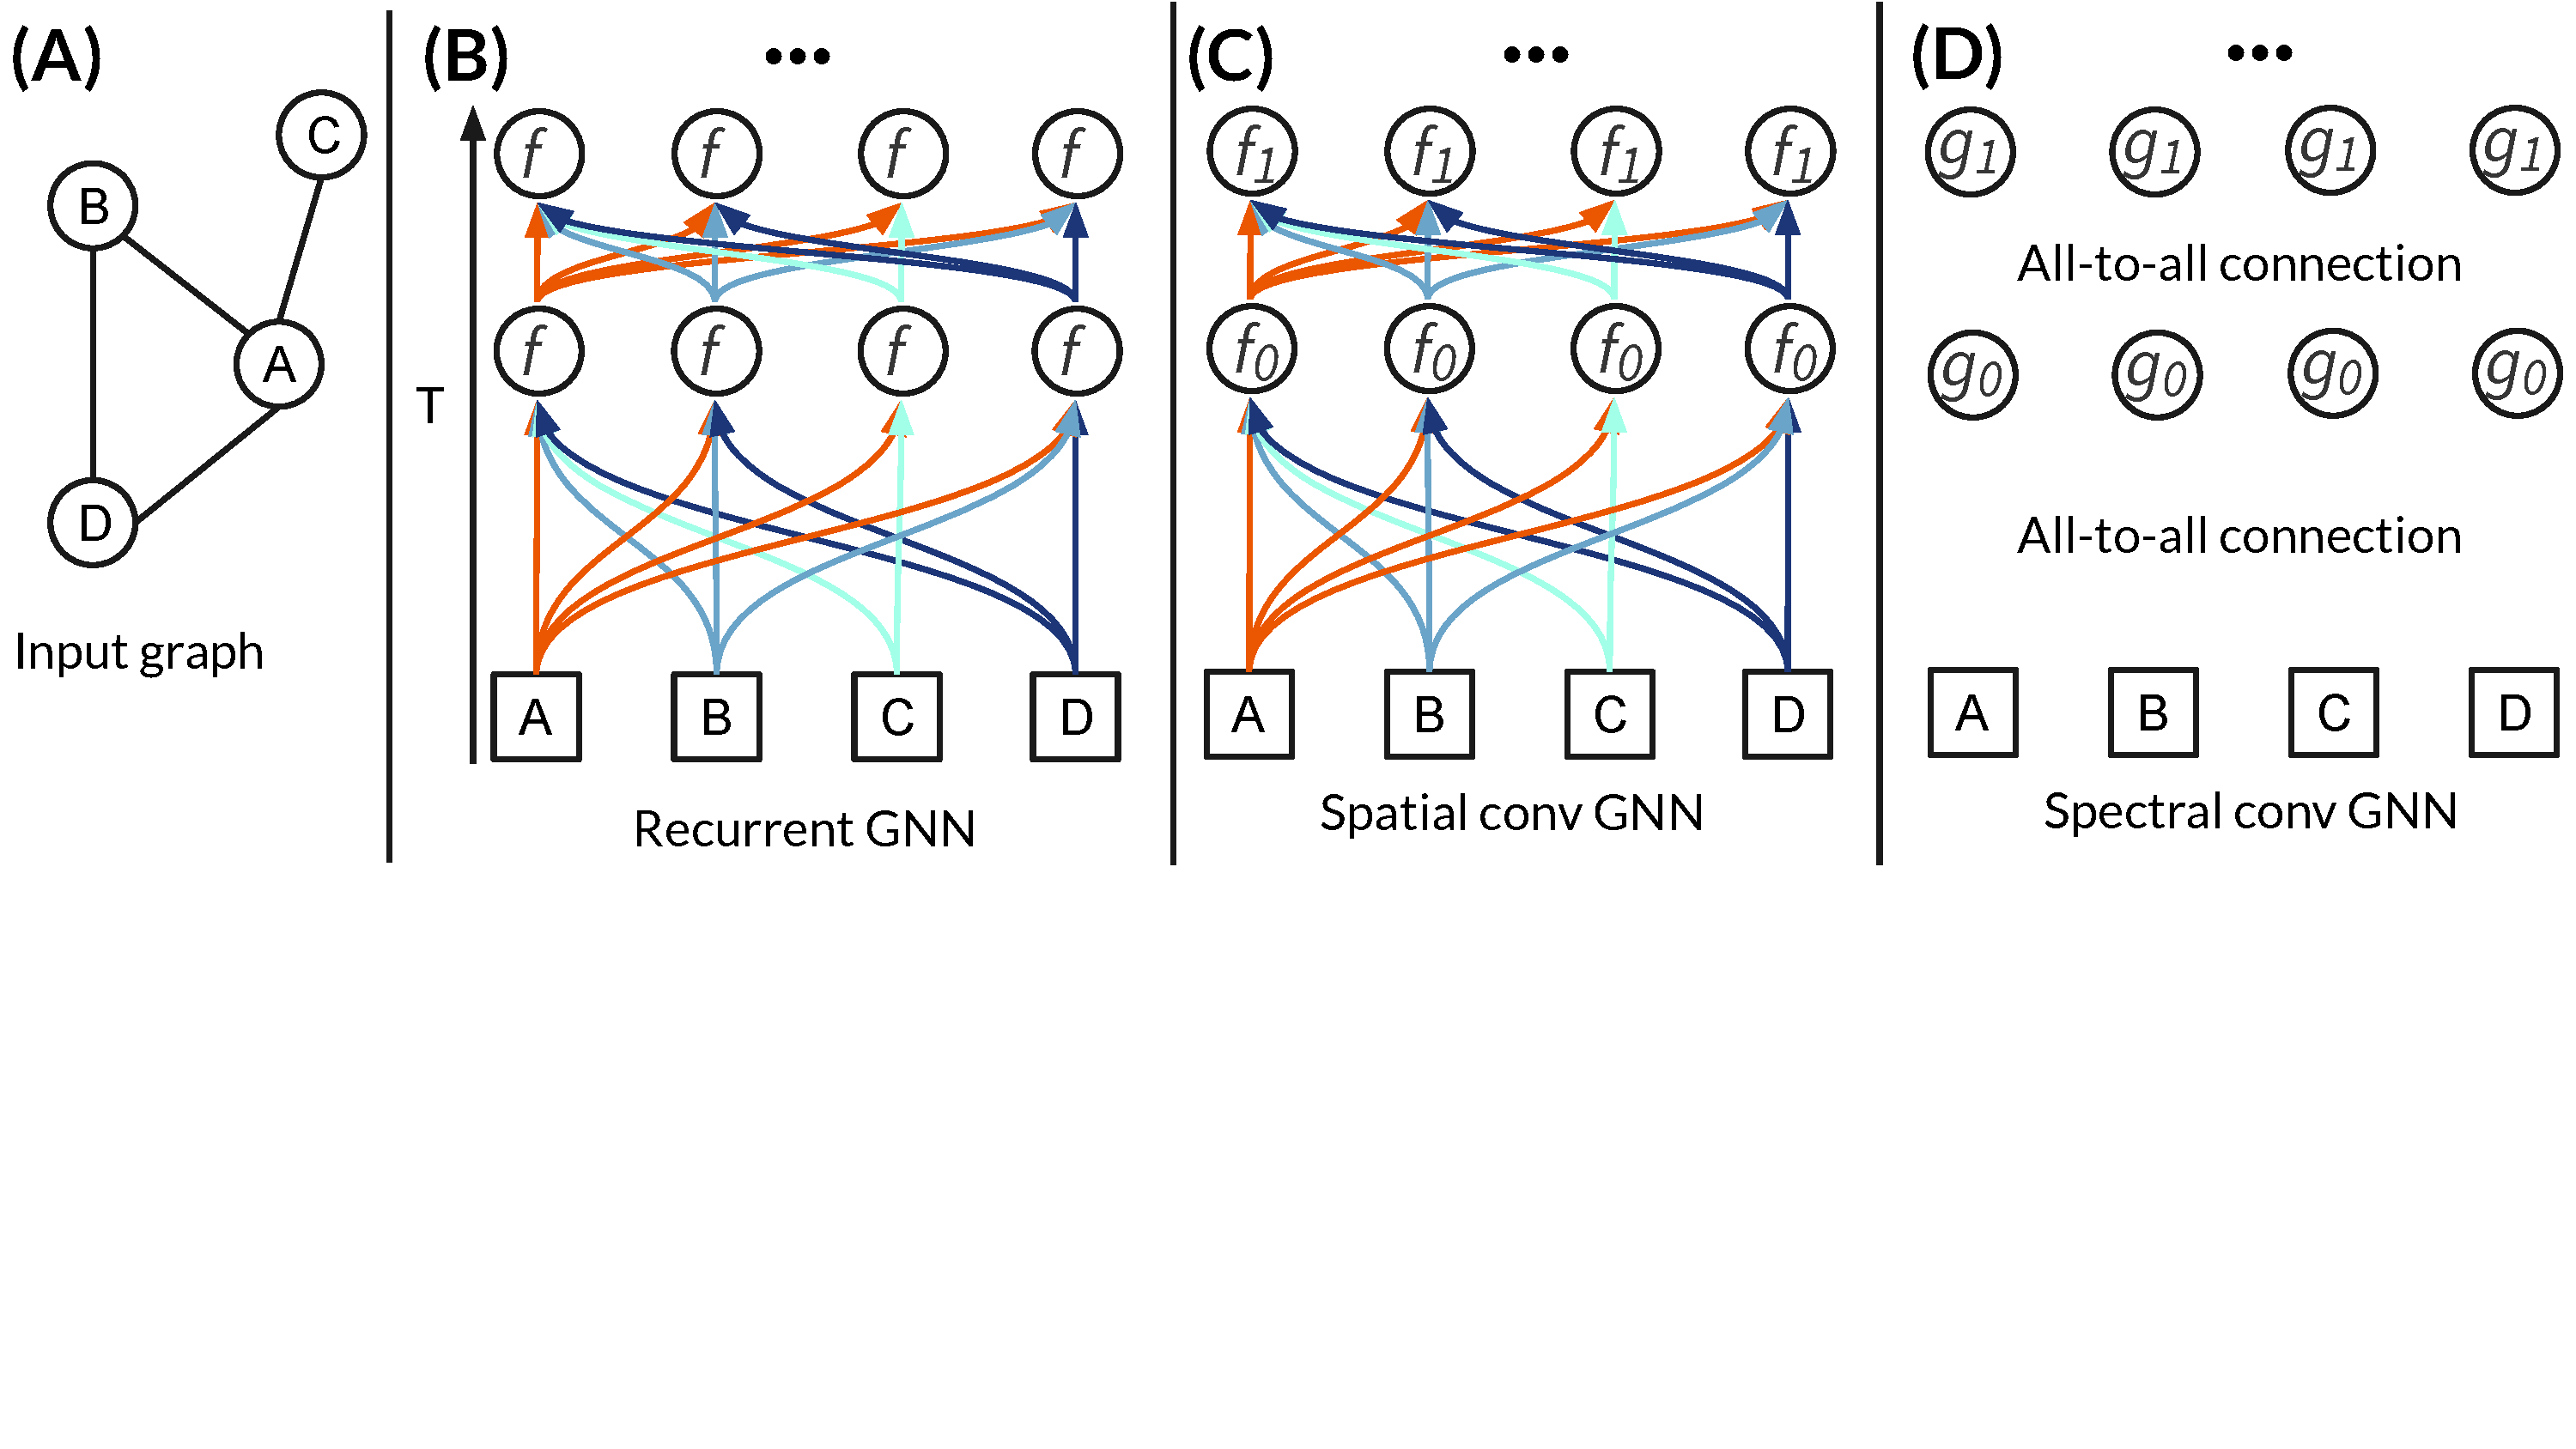
\includegraphics[width=0.75\textwidth]{./images/conceptual.pdf}
 \caption{Conceptual comparison of GNN architectures. (A): Input graph. (B): Recurrent GNN. Same function is applied recursively through time. (C): Spatial-based convolution. Different filters are applied in different layers. (D): Spectral-based convolution. Filters operate on the entire graph, unlike locally in (B) and (C).}
 \label{fig:conceptual}
\end{figure*}

\vspace{-2mm}
\section{Graph Neural Networks}\label{sec:gnn}
We now go over some representative graph neural network architectures. Roughly speaking, there have been three major branches of GNN: the recurrent GNN, the spatial-based convolutional GNN, and the spectral-based convolutional GNN. The first two types exploit spatial locality information in a graph. Therefore they are also collectively called the spatial method. In contrast, the latter one is called the spectral method, as it conducts graph convolution through a point-wise product in the graph Fourier space, based on the convolutional theorem. Such Fourier transform requires global information of the graph. Figure~\ref{fig:conceptual} shows a conceptual comparison between these methods.

Beyond spatial and spectral methods, there also exist other GNN architectures such as graph generative adversarial networks (Graph Autoencoders and GANs)~\cite{gae, ggan} and spatial-temporal GNNs~\cite{gaan, stgnn}. However, there are overlaps between them and spatial/spectral methods, and many of these architectures rely on primitives such as graph convolution. Due to space limits, this paper will focus on the spatial and spectral methods, as they are deemed more fundamental.


\subsection{Recurrent GNNs}
Recurrent GNNs are analogous to the Recurrent Neural Networks (RNNs) in the sense that they both contain a recursive neural network layer and apply the same set of parameters to different parts of the input data. Many of the first published works of GNN~\cite{gnn0} falls into this category, and there have been numerous subsequent works~\cite{gesn, ggnn, sse}. In the original paper, the architecture is simply named GNN, and in this survey, we will call it GNN-0 to differ from other GNNs.
\subsubsection{The Graph Neural Network Model (GNN-0)}\hfill \\
GNN-0~\cite{gnn0} is commonly known as one of the first works on graph neural networks. It calculates the hidden states of each node through a message passing/diffusion model, in which the hidden states of nodes are treated as information that can freely flow within the graph. Then each node's hidden state would finally reach equilibrium. Mathematically, the update rule for node $v$ at step $t$ can be written as:
\begin{gather}
\mathbf{h}_v ^t = \sum_{u \in \hat {\mathcal {N}}(v)} f(\mathbf{x_v}, \mathbf{x_u}, \mathbf{x_e}, \mathbf{h}_u^{t-1}),
\end{gather}
where $f$ is a learnable function and implemented using a fully connected neural network. For simplicity, if we stack all the node embeddings as column vectors to form matrices $\mathbf{H}_V^t$, and define a global transition function $F$ that is related to $f$, we can write:
\begin{gather}
\mathbf{H}_V^t = F(\mathbf{H}_V^{t-1})
\end{gather}
The graph's hidden states/node embeddings are said to be in equilibrium if:
\begin{gather}
\mathbf{H}_V^t = F(\mathbf{H}_V^{t-1}) = \mathbf{H}_V^{t-1}
\end{gather}
which indicates that the neural network does not further alter the hidden states of the node and that $\mathbf{H}_V^t$ is the fixed point of the function $f_w$. Additionally, another fully connected layer, denoted as function $g$, is added at the end of propagation to generate predictions based on the hidden states. The loss is then calculated based on the predictions and can be backpropagated to both $g$ and $f_w$ during training. The choice of using a multilayered neural network to implement $f$ and $g$ is convenient. However, this fixed point does not always uniquely exist unless if the function $f_w$ is a contraction map (Banach fixed-point theorem), a characteristic that a plain fully connected neural network does not possess. Therefore, to guarantee the uniqueness and existence of the fixed point, a correction term needs to be added to the loss function. This correction term would put constraints on the Jacobian of the neural network and consequently force it to be a contraction mapping.

GNN-0 resembles the form of a recurrent neural network, except it has a graph shape, while RNNs are list-like. Recurrent GNN has very similar characteristics with RNNs and shares the same training paradigm. A common practice is to unroll the GNN-0 in time, just like RNN, and Figure~\ref{fig:conceptual} (B) shows the unrolled network. The structure of the graph determines the connections between each layer. To train such a GNN model, common methods such as backpropagation through time (BPTT) can be adopted. However, the BPTT algorithm requires storing all the intermediate hidden states during the forward propagation, which drastically increases the memory footprint as the algorithm scales linearly with the number of layers. 

To overcome the memory issue of BPTT, GNN-0 adopts Recurrent Back-propagation (RBP), also known as the Almeida-Pineda algorithm~\cite{almeida, pineda}. RBP is a method for recurrent neural network training, and it is applicable when the hidden states of the recurrent neural network converge to a fixed point, which GNN-0 exactly does. RBP has a significant memory footprint reduction compared to BPTT as it stores only the hidden states of the last layer of recursion, meaning constant space complexity on a given graph and independent of the recursion depth. RBP works as follows iteratively: it first conducts a recursive forward propagation until the network reaches equilibrium. Then instead of unrolling the network in time, it conducts a recursive backpropagation until the gradients also become stable. It then applies the gradients and repeats for the next iteration.

Even with RBP to control the memory footprint, GNN-0 still faces various issues: as a recurrent neural network, it has the same problems RNNs face. It also conducts gradient descent (GD) that needs the whole graph and all hidden states for each iteration, while the de-facto deep learning training framework is stochastic gradient descent (SGD). Existing systems are mostly optimized for SGD training~\cite{cerebro, tf, torch, horovod}. There are attempts to apply SGD to recurrent GNN~\cite{sse}, but it is unknown if it still theoretically guarantees convergence to a fixed point. Furthermore, the constraint of contraction map GNN-0 was pointed out that it may hinder the expressive power of the neural network and may cause dropped performance for long-range dependencies~\cite{ggnn}.

\subsubsection{Gated Graph Neural Network (GG-NN)}\hfill \\
GG-NN~\cite{ggnn} is a follow-up work to GNN-0. It applies a gated recurrent unit (GRU) to construct the update rule of hidden states. Because of this, GG-NN does not guarantee a fixed point anymore and there is no need for the neural network to be contraction mapping. For the same reason, GG-NN requires an initialization the node embeddings, which are chosen to be the node features. GNN-0 does not need such initialization since the exponentially quick convergence is guranteed. The update rule of GG-NN can be written as:
\begin{gather}
\mathbf{h}_v ^0 = \mathbf{x}_v, \\
\mathbf{a}_v^t = \sum_{u \in \hat {\mathcal {N}}(v)} w_{e_{uv}} \mathbf{h}_u^{t-1},\\
\mathbf{h}_v^t = GRU(\mathbf{a}_v^t ),
\end{gather}
where $w_{e_{uv}}$ represents the parameter associated with the edge $e_{uv}$, this parameter is also learnable and depends on the type and direction of the edge. GG-NN updates the node embedding by first aggregating the embeddings of neighbors and then conducts a regular GRU operation on the aggregated results, defined as:
\begin{gather}
\mathbf{z}^t = \sigma(\mathbf{W}_z\mathbf{a}_v^t + \mathbf{U}_z\mathbf{h}_v^{t-1} ) \label{eq:updateg},\\
\mathbf{r}^t = \sigma(\mathbf{W}_r\mathbf{a}_v^t + \mathbf{U}_r\mathbf{h}_v^{t-1} ) \label{eq:resetg},\\
\mathbf{c}^t = \sigma(\mathbf{W}_c\mathbf{a}_v^t + \mathbf{U}_c(\mathbf{r}^t \odot \mathbf{h}_v^{t-1}) ) \label{eq:currentg},\\
GRU(\mathbf{a}_v^t) = (1 - \mathbf{z}^t ) \odot \mathbf{h}_v^{t-1} + \mathbf{z}^t \odot \mathbf{c}_v^{t}.
\end{gather} 
Equation~(\ref{eq:updateg}), (\ref{eq:resetg}), and (\ref{eq:currentg}) correspond to the update gate, reset gate, and current memory content of a GRU~\cite{gru}, respectively. $sigma$ is the sigmoid function; $\mathbf{W}_z, \mathbf{W}_r, \mathbf{W}_c, \mathbf{U}_z, \mathbf{U}_r, \mathbf{U}_c$ are weights associated with each gate. This grants GG-NN the capability of capturing long-range dependencies, and it relaxes the contraction mapping constraint. It still shares the same form as GNN-0. GG-NN then adopts truncated BPTT for training. Truncated BPTT can also avoid the potentially uncontrolled number of recursion steps as encountered in GNN-0. 

The most considerable modification of GG-NN to GNN-0 is the adoption of GRU with the size-fixed layer unrolling. This work removes the confinement for contraction mapping and mitigates the long-range dependency problems. However, without the theoretical guarantee of equilibrium, RBP becomes unsuitable for the task, and BPTT is used instead. This then increases this method's memory footprint, and one can see a subtle trade-off between GG-NN and GNN-0.




\subsection{Spatial-based Convolutional GNNs}
\label{sec:spatial}
Analogous to image convolutions, it is possible to generalize the definition of convolution to the graph domain. Spatial-based convolutional GNNs share a lot in common with recurrent GNNs. They mainly differ as the spatial methods use \textbf{different} filters in each layer, while in the recurrent GNNs, the same layer of neural networks are applied to the graph until an equilibrium (GNN-0) or a limited number of steps (GG-NN) is reached. This difference is illustrated as in Figure~\ref{fig:conceptual} (B) and (C).

Convolutional neural networks (CNNs) have proven successful in capturing shift-invariant local information and features of images. Suppose we treat an image as a graph and see each spatial location as a graph node and the pixel values (or the multi-channel feature vector, as in the intermediate layers) as the node embedding. In that case, a convolution on it can be seen as an aggregation of neighbor embeddings. We now give an example of how one could generalize image convolution to graph convolution. 

\vspace{2mm}
\noindent \textbf{Image convolution.} The convolution on an image $I(x, y)$ by a weighted filter $\omega(x,y)$ with size $a \times b$ is defined as:
\begin{gather}
I'(x, y) = \omega(x, y) \ast I(x, y) = \sum_{dx = -a}^{a}\sum_{dy=-b}^{b}\omega(dx, dy)I(x + dx, y + dy),
\end{gather}
where $I'(x, y)$ is the filtered image. This operation can be thought as first flipping the image both horizontally and vertically, then `sliding' the filter on the image to conduct point-wise product followed by sum. We now give an example. Let $I(x, y)$ to be an $5 \times 5$ single-channel image. We first flip it and it results in $\tilde I(x, y)$ and we explicit write out the pixel values of the $[2, 2]$ subimage of $\tilde I(x, y)$:
\begin{gather}
\tilde I= \left(
\begin{array}{ccccc}
 p_0 & p_1 & p_2 & \text{pixel} & \text{pixel} \\
 p_3 & p_4 & p_5 & \text{pixel} & \text{pixel} \\
 p_6 & p_7 & p_8 & \text{pixel} & \text{pixel} \\
 \text{pixel} & \text{pixel} & \text{pixel} & \text{pixel} & \text{pixel} \\
 \text{pixel} & \text{pixel} & \text{pixel} & \text{pixel} & \text{pixel} \\
\end{array}
\right),
\end{gather}
and a $3 \times 3$ filter $\omega(x, y)$ be written as: 
\begin{gather}
\omega = \left(
\begin{array}{ccc}
 w_0 & w_1 & w_2 \\
 w_3 & w_4 & w_5 \\
 w_6 & w_7 & w_8 \\
\end{array}
\right).
\end{gather}
Then after the filtering, the value at the location $(1, 1)$ of the filtered image is:
\begin{gather}
\label{eq:conveg}
I'(1, 1) = p_0 w_0 + p_1 w_1 + p_2 w_2 + ... = \sum_{i = 0}^8 p_i w_i.
\end{gather}
Note this is exactly a weighted sum of the pixel values surrounding spatial location $p_4$. The shape and size of the filter defines the scope of this summation. Now if we consider the image to be a graph, and each spatial location represents a node with the pixel value being the node feature, and add an edge from each node to its surrounding nodes (including diagonal and anti diagonal), we can rewrite Equation~\ref{eq:conveg} to be:
\begin{gather}
I'(1, 1) = \sum_{i \in \mathcal {N}((x, y))} p_i w_i,
\end{gather}
or in general:
\begin{gather}
I'(x, y) = \sum_{i \in \mathcal {N}((x, y))} p_i w_i.
\end{gather}
If the image is multi-channel, meaning each spatial location has, instead of a scalar, a vector of pixel values. The convolution can be written as:
\begin{gather}
\label{eq:imgconv}
I'(x, y) = \sum_{i \in \mathcal {N}((x, y))} \mathbf{p}_i \mathbf{w}_i.
\end{gather}
With this convenient form, we may now move on to define the spatial graph convolution in analogy. However, there are two distinctions between an image and a graph: 1. image nodes have a fixed number of neighbors, defined by the filter. 2. image node neighbors have an implicit ordering, also defined by the ordering of the filter. In a graph, the number of neighbors could vary from node to node, and the neighbors may be unordered (not positional). 

For graphs where we can safely assume a maximum degree and the ordering of the neighbors can be defined, we may be able to define graph convolution similarly to image convolution, but this may not work for general graphs. Moreover, in some applications, compared to the ordering of neighbors, one may care more about the types of edges connecting these neighbors. Hence, edge features may serve as a way to distinguish between neighbors, and naturally, we would want to share the filter weights for the same type of edges throughout the graph. 





\subsubsection{Neural Network for Graph (NN4G)} \hfill \\
NN4G~\cite{nn4g} was among the first works to introduce convolution operation on a graph. When it comes to the definition of graph convolution, it is tempting to try to use the definition in Equation~\ref{eq:imgconv}. However, as mentioned above, this definition would require the graph to be positional, and each node has a fixed degree. If we relax the requirements of a fixed degree but assume that there is a finite set of edges (the edges could be distinguished by the edge features, their directions, or by order in positional graphs), we can then share the weights within each edge type. This is called the stationary assumption. The definition in this scenario is as follows.

\vspace{2mm}
\noindent \textbf{Spatial graph convolution with stationarity assumption.} The convolution of a filter $\omega$ on a graph $G$ is defined as:

\begin{gather}
(\omega \ast \mathbf{X}_V) (v) = \sum_{u \in \mathcal {N}(v)} \mathbf{w}_{e_{uv}} \mathbf{h}_u,
\end{gather}
where $\mathbf{w}_{e_{uv}}$ is a learnable per-edge type vector of weights. Note this form is very similar to GG-NN's way of handling positional information. However, this definition of convolution is not applicable to general graphs where the edges are indistinguishable from each other. Therefore, NN4G uses a simplified but more general definition for convolution.

\vspace{2mm}
\noindent \textbf{General spatial graph convolution.} Without the stationary assumption, convolution is defined as:
\begin{gather}
(\omega \ast \mathbf{X}_V) (v)= \mathbf{w} \sum_{u \in \mathcal {N}(v)} \mathbf{h}_u,
\end{gather}
where $\mathbf{w}$ is a learnable weights vector shared for all edges and nodes. The contributions from the neighbors are summed together directly, as the edges are assumed to be indistinguishable. 

Based on the general spatial graph convolution, we can now go on to define the update rule of each node's hidden states:
\begin{gather}
\label{eq:nn4g}
\mathbf{h}_v ^k = \mathbf{W}_V^k~\mathbf{x}_v + \mathbf{W}_U^k \sum_{u \in \hat {\mathcal {N}}(v)} \mathbf{h}_u^{k-1},
\end{gather}
where $\mathbf{W}_V^k$ is the k-th layer weight matrix associated with the node features while $\mathbf{W}_U^k$ is the weight matrix associated with the aggregated neighbor features. Obviously, this update rule is incomplete until we add an activation function to operate on the right hand side. For the sake of simplicity, we omit all the activation functions from update rules from now on.

Commonly, the update rule can be re-written in matrix form to express the convolution on the entire graph:
\begin{gather}
\label{eq:nn4gm}
\mathbf{H}_V^k = \mathbf{W}_V^k~\mathbf{X}_V + \mathbf{W}_U^k \mathbf{H}_V^{k-1} \mathbf{A} ,
\end{gather}
where $\mathbf{H}_V^k$, $\mathbf{H}_V^{k-1}$, and $\mathbf{X}_V$ are stacked up horizontally (each vector forms a column in the matrx) by $\mathbf{h}_v ^k$, $\mathbf{x}_v$, and $\mathbf{h}_u^{k-1}$, respectively. $\mathbf{A}$ is the adjacency matrix.

Similar to recurrent GNNs, NN4G uses another neural network to generate predictions based on the extracted node embeddings, the loss of which is then backpropagated for training. Unlike the recurrent GNNs, NN4G contains only feed-forward neural networks, and neither BPTT nor RBP is needed. However, like GG-NN, it contains a fixed number of layers, and it needs to keep all intermediate hidden states for backpropagation, and the memory footprint could be high. 

NN4G and other spatial-based convolutional GNN are closely related to the recurrent GNNs. Collectively, they are called spatial methods as they directly work on the graph locally and extract the spatial information, in contrast to the spectral methods, which we will go over later. They are also designed to capture the shift-invariant features through weight sharing at different spatial locations. The major difference between them is spatial convolutional GNNs use multiple layers of different filters to gradually extract, ideally, higher-level features, whereas recurrent GNNs apply the same layer recurrently with the assumption of information propagation and equilibrium. 

\subsubsection{GraphSage} \hfill \\
So far, all methods we covered relied on batch gradient descent, in a sense that the entire graph must be iterated before one step of updates can be made to the model. This can hinder the training efficiency and scalability dramatically as the graph could be excessively large. More importantly, it could lead to many memory-related issues as the intermediate results of the entire graph need to be present before backpropagation.

GraphSage~\cite{graphsage} can mitigate these challenges. It proposes a batched training scheme through fix-sized sampling of the neighbors during each aggregation. The update rule for a spatial convolutional GNN can be written as:
\begin{gather}
\label{eq:graphsage}
\mathbf{h}_v ^k = \mathbf{W}_V^k~\mathbf{x}_v + \mathbf{W}_U^k \sum_{u \in \mathcal{S}(\hat {\mathcal {N}}(v))} \mathbf{h}_u^{k-1}.
\end{gather}
The summation can be substituted with any commutative and associative aggregation.

It then goes on to adopt the mini-batch SGD for training. During a training iteration, it first samples a batch of nodes to serve as the root nodes and fetch all of their k-hop neighbors, from which the node embedding will be extracted, and losses will be calculated. Then during the forward propagation, it keeps each aggregation size fixed by sampling the neighbors. With this tweak to the update rule, GraphSage has constant time and space complexity on a fixed graph architecture. 

\vspace{2mm}
\noindent \textbf{Neighbor explosion problem.} Through sampling, GraphSage can outperform prior arts by up to 100x~\cite{graphsage}. However, the challenge has not been fully solved. GraphSage still requires storing all of the related neighbors of the root node during training for each batch. With just one convolution layer, a fix-sized sample of all the 1-hop neighbors' features needs to be stored. This is a relatively small and constant amount of data and can be handled easily. Then if we propagate to the second convolution layer, we will then need to calculate each 1-hop neighbor's node embedding generated by the first layer, which will then require storing their 1-hop neighbors as well. This indicates we will need to store in total the k-hop neighbors of one root node to calculate its embedding after the k-th layer. The size of memory consumption grows exponentially with the number of layers and can hinder the scalability. This issue is referred to as the neighbor explosion problem~\cite{neiexplode}. 

\subsubsection{Fast Learning with Graph Convolutional Network (FastGCN)} \hfill \\

Sampling proves to be a somewhat effective tool when handling scalability issues. However, GraphSage's neighbor sampling is still subject to the neighbor explosion problem. As the depth of the GNN increases, the sampled subgraph exponentially grows, and it can quickly become a large portion of the original graph, diminishing the goal of reducing the memory footprint. This problem stems from the fact that the graph data is non-i.i.d. A sampling of vertices will also involve their neighbors. 

FastGCN~\cite{fastgcn} proposes to improve the efficiency and scalability of spatial convolutional GNN by introducing an i.i.d. assumption and then samples the original graph nodes as if they were independently drawn from a distribution. It draws random sampling in each convolutional layer and this can be seen as an approximation to convolution. The update rule is written as:
\begin{gather}
\mathbf{h}_v ^k = \mathbf{W}_V^k~\mathbf{x}_v + \mathbf{W}_U^k \sum_{u \in \hat {\mathcal {N}}(v) \land u \in \mathcal{S}^{k-1}(V)} \mathbf{h}_u^{k-1}, if~v \in \mathcal{S}^{k}(V),
\end{gather}
where $\mathcal{S}^{k-1}(V)$ is the sampled nodes in the k-th layer. If $v \notin \mathcal{S}^{k}(V)$, $\mathbf{h}_v ^k$ will not be calculated. 

With this sampling of nodes, time and space complexity now become the summation of sample sizes of every layer and therefore linear, instead of exponential, to the number of layers. On the other hand, this sampling is radical, and the inter-connections between layers could be scarce as each node has an independent sample of nodes, which may or may be connected with the previous and next layer's sample. 



\subsection{Spectral-based Convolutional GNNs}
\label{sec:spectral}
Spectral-based convolutional GNNs, or simply spectral GNNs, are stemmed from the world of graph signal processing and have many theoretical backgrounds. They usually assume the graph to be undirected. Instead of defining graph convolution analogous to image convolutions, these GNNs conduct convolution relying on the convolution theorem. It has been shown in~\cite{gcn} that after a series of approximation and normalization, spectral-based methods can also be reduced to spatial-based methods. 

\subsubsection{Spectral-based Convolutional GNN} \hfill \\

Spectral-GNN~\cite{spectralgnn} was one of the first spectral-based GNNs. 
We now have a closer look at how spectral-based methods work. They treat the node features $\mathbf{X}$ as graph signal and define a Fourier transform based on the structure of the graph. Let deg$(v)$ be a function to return the degree of node $v$. Given the adjacency matrix of the graph $\mathbf{A}$, define the node degrees matrix to be a diagonal matrix $\mathbf{D}$:
\begin{gather}
\mathbf{D}_{ii} = \sum_j \mathbf{A}_{ij} = \text{deg}(v_{ij}). 
\end{gather}
Then define the symmetric normalized Laplacian of the graph to be:
\begin{gather}
\mathbf{L} = \mathbf{I} - \mathbf{D}^{-1/2}\mathbf{A}\mathbf{D}^{-1/2},
\end{gather}
where $\mathbf{I}$ is a unit matrix. Graph Laplacian is a matrix representation of the graph. The element of it can be written as:
\begin{gather}
\mathbf{L}_{ij} =
  \begin{cases}
   1 & i=j ~\text{and}~ \text{deg}(v_{ij}) \ne 0,\\
   -\dfrac{1}{\sqrt{\text{deg}(v_i) \text{deg}(v_j)}} & i \ne j ~\text{and}~ v_j \in \mathcal{N}(v_i),\\
   0 & \text{otherwise}.
  \end{cases}
\end{gather}
Graph Laplacian is a real symmetric positive semidefinite. The eigendecomposition of $\mathbf{L}$ yields:
\begin{gather}
\mathbf{L} = \mathbf{Q}~\mathbf{\Lambda}~\mathbf{Q}^\intercal,
\end{gather}
where $\mathbf{Q}$ is an orthogonal matrix whose columns are the eigenvectors, and $\mathbf{\Lambda}$ is a diagonal matrix composed of the eigenvalues. $\mathbf{Q}$ is then used to define the graph Fourier transform on the graph signal (node features).

\vspace{2mm}
\noindent \textbf{Graph Fourier transform $\mathcal{F}$ and inverse transform $\mathcal{F}^{-1}$:}
\begin{gather}
\hat {\mathbf{X}}_V = \mathcal{F}(\mathbf{X}_V) = (\mathbf{Q}^\intercal~\mathbf{X}_V^\intercal)^\intercal = \mathbf{X}_V~\mathbf{Q},\\
\mathbf{X}_V = \mathcal{F}^{-1}(\hat {\mathbf{X}}_V) = \hat {\mathbf{X}}_V~\mathbf{Q}^\intercal,
\end{gather}
where $\hat {\mathbf{X}}_V$ is the transformed node features. Spectral methods then uses the convolution theorem to compute convolution given the Fourier transform. The spatial convolution on the graph signal can be expressed as a point-wise product in the spectral space. As of now, we start with a simplified single-channel scenario when $D_v$ = 1, then $\mathbf{X}_V \in \mathbb{R}^{1 \times |V|}$, i.e., row vector. Assume the filter to be $\mathbf{\Theta} \in \mathbb{R}^{1 \times |V|}$, we have the definition of convolution:

\vspace{2mm}
\noindent \textbf{Spectral graph convolution:}

\begin{gather}
\label{eq:spectralconv}
\begin{split}
\mathbf{\Theta} \ast \mathbf{X}_V & = \mathcal{F}^{-1}(\mathcal{F}(\mathbf{\Theta}) \odot \mathcal{F}(\mathbf{X}_V)) \\
& = ((\mathbf{\Theta}~\mathbf{Q}) \odot (\mathbf{X}_V~\mathbf{Q}))~\mathbf{Q}^\intercal,
\end{split}
\end{gather}
the output would also be in $\mathbb{R}^{1 \times |V|}$. To simplify it, we can define:
\begin{gather}
\hat {\mathbf{\Theta}} = \text{diag}(\mathbf{\Theta}~\mathbf{Q}),
\end{gather}
where diag(.) is function that maps a vector to a diagonal matrix. Then Equation~\ref{eq:spectralconv} can be re-written as:
\begin{gather}
\label{eq:spectralconvfin}
\mathbf{\Theta} \ast \mathbf{X}_V = \mathbf{X}_V~\mathbf{Q}~\hat{\mathbf{\Theta}}~\mathbf{Q}^\intercal.
\end{gather}
This already gives us a way to calculate the convolution on only one of the channels, we now generalize it to multiple channels and filters~\cite{spectralgnn}. The update rule can be written as:
\begin{gather}
\begin{split}
\mathbf{H}^k[c, :] & = \sum_i \mathbf{\Theta}^{c, i, k} \ast \mathbf{H}^{k - 1}[i, :] \\
& = \sum_i \mathbf{H}^{k - 1}[i, :]~\mathbf{Q}~\hat{\mathbf{\Theta}}^{c, i, k}~\mathbf{Q}^\intercal,
\end{split}
\end{gather}
where $\hat{\mathbf{\Theta}}^{c, i, k}$ is in the $k$-th layer, the $c$-th filter's sub-filter that operates the $i$-th channel of the previous layer's outputs. 

\vspace{2mm}
\noindent \textbf{Comparison between spatial and spectral methods:}
It can be seen that spectral-based convolution is a global operation that is defined on a per-channel basis. For each input channel, there is an associated filter that operates on the entire graph. Filtered results from each previous channel are summed together to form one output channel. Thus, for each convolution, it requires the entire graph to calculate. This is drastically different from the spatial methods, which operate on spatial locations and share the filter weights. 



Despite their theoretical importance, spectral methods have many issues that limit their efficiency and scalability. There are three major drawbacks :
\begin{enumerate}
\item Requirements for eigendecomposition. Eigendecomposition, generally speaking, is a costly $O(|V|^3)$ operation, and it requires access to the entire graph at the training time, which may not be feasible, sometimes not even possible.
\item Graph Fourier transform is graph-dependent, meaning knowledge transfer from an existing graph to new nodes or to a completely new graph is non-trivial.
\item Difficult to apply to dynamic graphs. Adding or deleting nodes from the graph would trigger a recalculation of the eigendecomposition and retraining of the GNN.
\end{enumerate}

Due to these constraints, spatial methods are generally more scalable and flexible than spectral methods. 
\subsubsection{ChebNet and Graph Convolutional Networks (GCN)} \hfill \\
ChebNet~\cite{chebnet}, local spectral-GNN~\cite{hammond}, and GCN~\cite{gcn} are among the works that attempt to simplify spectral method via approximation, because of the issues mentioned above. 

We can approximatee the global filter by Chebyshev polynomials of $\mathbf{\Lambda}$, an approximation approach introduced in~\cite{hammond, chebnet}, so that the filters are no long global. The convolution can be approximated as K-truncated Chebyshev polynomials:
\begin{gather}
\hat {\mathbf{\Theta}} \approx \sum_i^K \theta_i T_i(\mathbf{\Lambda}),
\end{gather}
where $\theta_i$ is learnable weight and $T_i$ is the Chebyshev polynomial, defined as: $T_i(x) = 2xT_{i-1}(x) - T_{i-2}(x), T_0(x) = 1, T_1(x) = x$. Plug it in Equation~\ref{eq:spectralconvfin}, we can obtain:
\begin{gather}
\mathbf{\Theta} \ast \mathbf{X}_V = \mathbf{X}_V~\sum_i^K \theta_i T_i(\mathbf{L}),
\end{gather}
where the multiplication with $\mathbf{Q}$ and $\mathbf{Q}^\intercal$ have been absorbed in to $L$, saving a $O(|V|^2)$ matrix multiplication. Meanwhile, now the polynomial becomes about the Laplacian and only up to order $K$, this also implies locality, based on a lemma~\cite{hammond}:

\vspace{2mm}
\noindent \textbf{Lemma 1.} \textit{Let $\mathbf{L}$ be the graph Laplacian (normalized or non-normalized) and $s$ > 0 an integer. For any two nodes $m$ and $n$, the length of the shortest path between $m$ and $n$ is larger than $s$, then $\mathbf{L}^s_{mn} = 0$}.

Therefore, for any node that is more than $K$-hop away from a given central node of convolution, it does not contribute since the Laplacian is zero, and therefore this convolution becomes local.

Furthermore, if we take only $K=1$ and assume $\theta_0 = \theta_1 = \theta$, we have~\cite{gcn}:
\begin{gather}
\mathbf{\Theta} \ast \mathbf{X}_V =\theta \mathbf{X}_V (\mathbf{I} + \mathbf{D}^{-1/2}\mathbf{A}\mathbf{D}^{-1/2}).
\end{gather}
The scope of convolution will then be limited to only the 1-hop neighbors. Now if we enable multi-channel input and upgrade $\theta$ to be a matrix $\bar {\mathbf{\Theta}}$ consisting of multiple filters, and define $\bar {\mathbf{A}} = \mathbf{I} + \mathbf{D}^{-1/2}\mathbf{A}\mathbf{D}^{-1/2}$, the update rule can be written as:

\begin{gather}
\mathbf{H}_V^k = \bar {\mathbf{\Theta}}^k~\mathbf{H}_V^{k-1} \bar {\mathbf{A}},
\end{gather}
which shares the same form of Equation~\ref{eq:nn4g}, except for the normalized adjacency matrix $\bar {\mathbf{A}}$, which can improve the numerical stability of GCN. Finally, we are able to draw the connection between spectral methods and spatial methods and unify them under the same framework. Spatial methods can be seen as a first-order approximation of the spectral methods.
\begin{figure*}[t]
 \centering
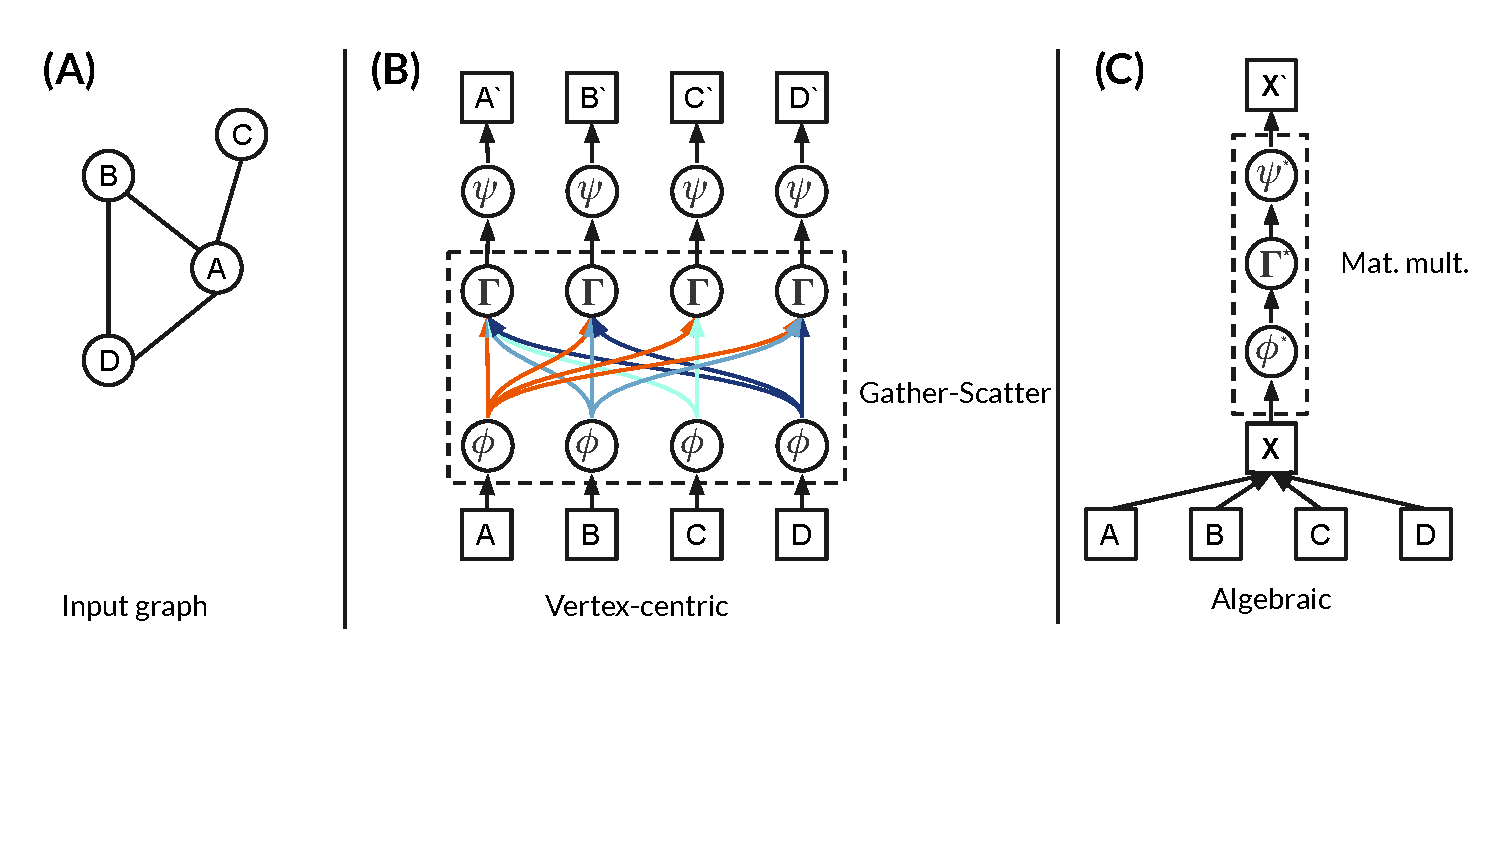
\includegraphics[width=0.70\textwidth]{./images/gnnsys.pdf}
 \caption{An example of two different approaches for GNN execution. (A): Input graph. (B): Vertex-centric approach. (C): Algebraic approach.}
 \label{fig:ggnnsys}
\end{figure*}

\section{GNN Systems} \hfill \\
\label{sec:gnnsys}
So far, we have seen that GNNs are largely related to classical deep learning methods such as CNN or RNN. However, the graph data structure adds complexity as graph data can be irregular and connected explicitly. To apply to irregular data and capture a graph's structural information, various GNNs have been proposed. 

Now a natural question is: \textit{how do we build software systems to support the GNN-based graph analytics better?} And most importantly, with training/inference being the most computationally intensive part, \textit{how do we build more efficient and scalable systems for GNN training/inference}? In the past, a huge amount of effort has been put into general ML systems for classical deep learning. Most of theese are dataflow systems~\cite{spark, tf, torch}. Now it is time to consider how to re-use or develop new techniques for scalable and efficient graph deep learning. As an emerging topic, GNN system is gradually gaining popularity. 

As of now, most of the GNN system research mainly focus on the spatial methods. Majority of spatial methods can be expressed via a general update rule:
\begin{gather}
\label{eq:mmp}
\mathbf{h}_v ^k = \psi ( \mathbf{x}_v^k, \gammasum_{u \in {\mathcal {N}}(v)}  \phi(\mathbf{h}_v^{k-1}, \mathbf{h}_u^{k-1}, \mathbf{x}_{e_{vu}})),
\end{gather} 
where $\psi$, $\phi$, $\Gamma$ are potentially learnable and differentiable functions, $\Gamma$ is further required to be commutative and associative. $\psi$ is called the update function, $\phi$ the message function and $\Gamma$ the aggregate function.


%\subsubsection{NeuGraph} \hfill \\
%One natural way to support GNNs in a dataflow system is to represent the GNN as a DAG and provide it to the existing system. However, it often requires loading a large amount of data into the very limited GPU memory because of the aforementioned neighbor explosion problem. And there are graph-specific optimizations that the dataflow systems would not exploit. NeuGraph~\cite{neugraph} is a system built to provide better support for GNN on top of dataflow systems.

\subsubsection{PyTorch Geometric (PyG) and NeuGraph} \hfill \\
Equation~\ref{eq:mp} fits in the paradigm of vertex-centric programming, which is a common programming model in the graph processing world~\cite{vertexcentric, powergraph, pregel} and very easy to parallelize. PyG~\cite{pyg} follows this pattern and builds GNNs as dataflow graphs on top of PyTorch~\cite{torch}, a dataflow system. Figure~\ref{fig:gnnsys} (B) shows an example computational graph generated. Each (vectorized) operation is then put on a separate processor to achieve parallelism. Built on top of PyTorch, PyG can easily utilize the features PyTorch provides, such as autograd, GPU acceleration, etc. 

NeuGraph~\cite{neugraph} is another GNN system built on top of a dataflow system and designed for a single-node multi-GPU setting. It extends the GAS~\cite{powergraph} programming model and partitions the computational graph to avoid GPU OOM issues. It further exploits GPU-to-GPU communication to avoid latencies of GPU-to-DRAM. 

\subsubsection{Deep Graph Library (DGL)} \hfill \\
DGL~\cite{dgl} takes a different approach for the GNN execution, especially for the message passing (gather-scatter) part. It takes an algebraic approach for the execution by expressing GNN as sparse matrix multiplications (SpMM). This is analogous to those algebraic approaches to general graph analytics tasks~\cite{graphla}.

Figure~\ref{fig:gnnsys} (C) gives an example of the algebraic approach taken by DGL; each step is summarized as linear algebra and executed as SpMM, which is executed via DGL's own specialized kernel. DGL is built upon existing deep learning systems, and the user can also write user-defined functions to extend the built-in functions. DGL describes itself as a framework independent system, that is, independent of the underlying deep learning system. It has full support for several popular frameworks such as Tensorflow or PyTorch as backend. Backpropagation can also be done via another SpMM, and DGL functions are registered in the underlying deep learning framework to take advantage of autograd.

The algebraic approach opens possibilities of operator fusion. For instance, consider the update rule for NN4G in Equation~\ref{eq:nn4g}, it can also be represented as Equation~\ref{eq:nn4gm} with purely matrix multiplications. Note in this form, the message function can be fused together with the aggregation function, and there is no need to materialize the intermediate messages.


\vspace{2mm}
\noindent \textbf{Comparison between PyG and DGL.} Generally speaking, the vertex-centric approach has advantages on low-degree graphs, and when the graph data is not coalesced and data access could become a bottleneck for the algebraic approaches. On the contrary, algebraic approaches do not need to materialize the huge amount of messages, leading to system crashes. Algebraic approaches could fuse the message function with the aggregation, and DGL tends to perform better on higher-degree graphs.

 

\section{Conclusion and Discussion}
\label{sec:conclusion}
In this paper, we surveyed GNN research, ranging from pioneering works to milestone papers. GNN research is gaining enormous attention, and scalability and efficiency have been one of the major topics.
We now discuss the potential research directions on the scalability and efficiency of GNNs.

On the algorithmic research of GNNs. Sampling has proven to be a very effective way of increase GNN efficiency. However, graph sampling is non-trivial because of the non-i.i.d. nature of graph data. Moreover, ignoring the interconnections may lead to degraded accuracy performance. Therefore, sophisticated sampling that considers the connections while still offering a boost in efficiency and scalability is a very important problem. Similarly, graph coarsening, which distills the original graph to be smaller subgraphs, can also significantly improve efficiency.

On the GNN system research. One natural direction for GNN system research is to scale out, i.e., distributed processing, which is receiving attention. On the other hand, they face even more problems like graph partitioning and load balancing. As mentioned before, the graph data is non-i.i.d., thus both sampling and partitioning are difficult to do. Graph partitioning for GNN itself is already a hard problem, let alone considering load-balancing simultaneously. The other important direction is compilers that can generate fused kernels for GNN operations, given a set of arbitrary user-defined functions. Such innovation would be especially useful for algebraic approaches. Meanwhile, existing general-purpose graph analytics systems may have more to offer, especially on the front of scalability and when the system needs to operate on huge graphs.


%\input{experiments}
%\input{related_work}
%\input{discussion}
%\input{acknowledgement}


% \pagebreak
\bibliography{main}
\bibliographystyle{abbrv}
%</tag>
\end{document}
